\section{Model}
\label{sec:model}

\setlength{\tabcolsep}{2pt}
\begin{figure*}
\begin{center}
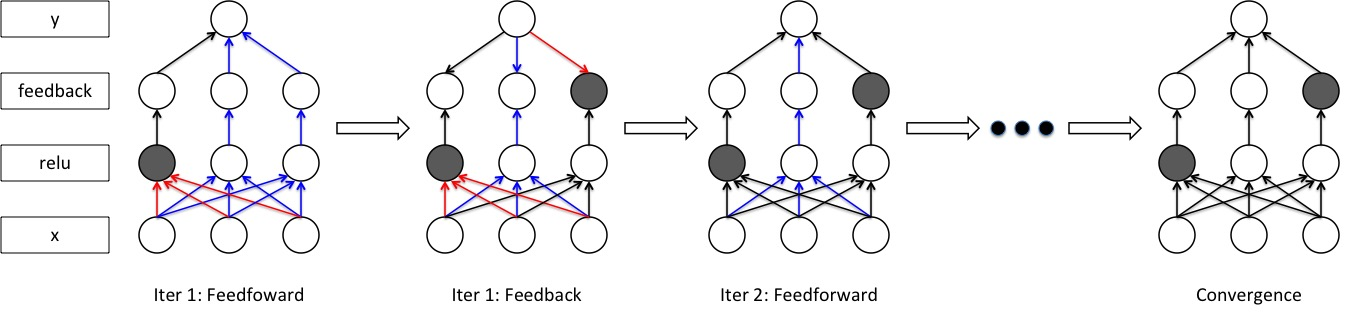
\includegraphics[width=0.95\linewidth]{figs/model/model}
% \vspace{-10pt}
\caption{Illustration of our feedback model and its inference process. At the first iteration, the model performs as a feedforward neural net. Then, the neurons in the feedback hidden layers update their activation status to maximize the confidence output of the target top neuron. This process continues until convergence. (We show only one layer here, but feedback layers can be tacked in the deep ConvNet.)}
\label{fig:model}
% \vspace{-30pt}
\end{center}
\end{figure*}
% I commented this paragraph
\begin{comment}
We first review the current state-of-the-art feedforward Deep Convolutional Neural Networks (CNNs) architecture and then propose our feedback model.
\end{comment}

\subsection{Review of Convolutional Neural Networks}
The most recent state-of-the-art deep CNNs~\cite{Simonyan2014Very} consist of many stacked feedforward layers, including convolutional, rectified linear units (ReLU) and max-pooling layers. For each layer, the input $\mathbf{x}$ can be an image or the output of a previous layer, consisting of $C$ input channels of width $M$ and height $N$: $\mathbf{x} \in \mathcal{R}^{M \times N \times C}$. The output $\mathbf{y}$ consists of a set of $C'$ output channels of width $M'$ and height $N'$: $\mathbf{y} \in \mathcal{R}^{M' \times N' \times C'}$.

\textbf{Convolutional Layer:}
The convolution layer is used to extract different features of the input. The convolutional layer is parameterized by $C'$ filters with every filter $\mathbf{k} \in \mathcal{R}^{K \times K \times C}$.
\begin{equation}
\mathbf{y}_{c'} = \sum_{c=1}^C \mathbf{k}_{c'c} * \mathbf{x}_c,\ \forall c'
\end{equation}

\textbf{ReLU Layer:}
The ReLU layer is used to increase the nonlinear properties of the decision function and of the overall network without affecting the receptive fields of the convoluional layer.
\begin{equation}
\mathbf{y} = \max (\mathbf{0}, \mathbf{x})
\label{eq:relu}
\end{equation}

\textbf{Max-Pooling Layer:}
The max-pooling layer is used to reduce the dimensionality of the output and variance in deformable objects to ensure that the same result will be obtained even when image features have small translations. The max-pooling operation is applied for every pixel $(i,j)$ around its small neighborhood $\mathcal{N}$.
\begin{equation}
y_{i,j,c} = \max_{u,v \in \mathcal{N}} x_{i+u, j+v, c},\ \forall i, j, c
\label{eq:max-pool}
\end{equation}

\begin{comment}
\textbf{Fully Connnected Layer:} The fully connected layer is parameterized by the production matrix with $W \in \mathcal{R}^{M'N'C' \times MNC}$.
Finally, a few fully connected layers (normally with drop-out) is stacked on top of the convolutional outputs to compute the scores of every class.
\begin{equation}
\vec{y}_l = W_l^T  \vec{y}_{l-1}
\end{equation}
\end{comment}

\subsection{Re-interpreting ReLU and Max-Pooling}

%The ReLU and max-pooling layers can be re-interpreted as components for feature selection in neural nets. During feedforward computation, ReLU and max-pooling layers select those neuron signals that are either \emph{confident enough or locally maximal} to facilitate the invariance~\cite{riesenhuber1999hierarchical} and spatial assignments~\cite{weng1992cresceptron} for messages passing to higher levels.

To better understand how selectivity works in neural networks and how to formulate the feedback, we re-interpret behaviors of ReLU and Max-Pooling layers as a set of binary activation variables $\mathbf{z} \in \{0,1\}$ instead of the $\max()$ operation in Equation~\ref{eq:relu}~and~\ref{eq:max-pool}. Thus, behaviors of ReLU and Max-Pooling could be formulated as $\mathbf{y} = \mathbf{z} \circ \mathbf{x}$, where $\circ$ is the element wise product (Hadamard product); and $\mathbf{y} = \mathbf{z} * \mathbf{x}$, where $*$ is the convolution operator and $\mathbf{z}$ is a set of convolutional filters except that they are location variant.

Be interpreting ReLU and Max-Pooling layers as ``gates'' controlled by input $x$, the network selects information during feedforward phases in a \emph{bottom-up} manner, and eliminates signals with minor contributions in making decisions. However, the activated neurons could be either helpful or harmful for classification, and involve too much noise especially for complex scenes.
%We introduce a set of binary activation variables $\mathbf{z} \in \{0, 1\}$ to replace the $\max()$ operations in these layers. For the ReLU layer, $\mathbf{z}$ is the same size as the input $\mathbf{x}$ and Equation~\ref{eq:relu} can be rewritten as $\mathbf{y} = \mathbf{z} \circ \mathbf{x}$, where $\circ$ is the element wise product (Hadamard product). For the max-pooling layer, $\mathbf{z}$ is a set of convolutional filters except that they are location variant. Equation~\ref{eq:max-pool} can be rewritten as $\mathbf{y} = \mathbf{z} * \mathbf{x}$, where $*$ is the convolution operator.

%For both layers, the $\max()$ functions are replaced with linear operations between the inputs and binary activation variables. The binary activation variables perform feature selection. However, the values of $\mathbf{z}$ are completely determined by the bottom-up input $\mathbf{x}$, meaning that the feature selections are purely based on bottom-up signals and won't be changed by any top-down information.

%During the feedforward process, the neural nets need to keep an overall description of the image content and make image feature representations as general as possible, due to the lack of top-down semantic information. To achieve this target, middle-level neurons try to turn enough ReLUs on to avoid information loss; while the high-level fully connected layers are responsible for providing discriminability and descriptive ability. This works well when there is only one salient object in the image and no prior information is given. However, when the image contains multiple objects and complex scenes, the same feature may be too general to work equally well for all objects.

% During the feedforward process, the neural net features need to keep a overall description of the image content, due to the lack of top-down global information. The middle-level neurons try to turn on enough ReLU on while the high-level fully connected layers try to keep the feature embedding as discriminative and descriptive as possible. This works well when there is only one salient object in the image and no prior information is given. However, when the image contains multiple objects and complex scenes, the same feature may be too general to work equally well for all objects.

\subsection{Introducing the Feedback Layer}
Since the model opens all gates and allow maximal information getting through to ensure the generalization, to increase the discriminability within feature level, it is feasible to turn off those gates that provide irrelevant information when targeting at particular semantic labels. This strategy is explained as selectivity in biased competition theory~\cite{desimone1995neural} and is critical to realize the top-down attention.
%when we are targeted on a particular semantic labels, we want to turn off those gates that provide irrelevant information for seeing that object. This top-down message will be utilized to turn off those relu.

More technically, to increase the model flexibility to images and prior knowledges, we introduce an extra layer to the existing convolutional neural network. We call it the \emph{feedback layer}. The feedback layer contains another set of binary neuron activation variables $\mathbf{z} \in \{0, 1\}$, in addition to ReLU. However, these binary variables are activated by top-down messages from outputs, instead of bottom inputs.
%
The feedback layer is stacked upon each ReLU layer, and they compose a hybrid control unit to active neuron response in both bottom-up and top-down manners:
\\\textbf{Bottom-Up} Inherent the selectivity from \emph{ReLU layers}, and the dominant features will be passed to upper layers;
\\\textbf{Top-Down} Controlled by \emph{Feedback Layers}, which propagate the high-level semantics and global information back to image representation. This is achieved by activating only those gates related with target neurons.
\\Figure.~\ref{fig:model} illustrates a simple architecture of our feedback model with only one ReLU layer and one feedback layer.

\begin{comment}
\begin{description}
  \item[Bottom-Up] Inherent the selectivity from \emph{ReLU layers}, and the dominant features will be passed to upper layers;
  \item[Top-Down] Controlled by \emph{Feedback Layers}, which propagate the high-level semantics and global information back to image representation. This is achieved by activating only those gates related with target neurons.
\end{description}
\end{comment}

\subsection{Updating Hidden Neurons in Feedback Loops}
Given an image $I$ and a neural network with learned parameters $w$, we optimize the target neuron output by jointly inference on binary neuron activations $\mathbf{z}$ over all the hidden feedback layers. In particular, if the target neuron is a $k$-th class node in the top layer, we optimize the class score $s_k$ by re-adjusting the neuron activations at every pixel $(i,j)$ of channel $c$, on feedback layer $l$.
\vspace{-3pt}
\begin{equation}
\begin{aligned}
& \max_\mathbf{z} & & s_k(I, \mathbf{z}) - \lambda ||\mathbf{z}|| \\
& s.t. & & \ z^l_{i,j,c} \in \{0, 1\}, \; \forall\ l, i, j, c
\end{aligned}
\end{equation}
\vspace{-5pt}

This leads to an integer programming problem, which is NP-hard given the current deep net architecture. An approximated solution could be derived by applying a linear relaxation:
\begin{equation}
\begin{aligned}
& \max_\mathbf{z} & & s_k(I, \mathbf{z}) - \lambda ||\mathbf{z}|| \\
& s.t. & & \ 0 \leq z^l_{i,j,c} \leq 1, \; \forall\ l, i, j, c\\
\end{aligned}
\end{equation}

We use the gradient ascent algorithm to update the hidden variables through all layers simultaneously.
\begin{equation}
\begin{aligned}
\mathbf{z}_{t+1} = \mathbf{z}_t + \alpha \cdot (\frac{\partial s_k}{\partial \mathbf{z}} |_{\mathbf{z}_t} - \lambda)
\end{aligned}
\end{equation}

The initialization of feedback layer status $z$ is set to be the corresponding ReLU activation after the first feedforward pass and truncate $z$ when the updated values are either larger than 1 or smaller than 0 during inference.

\subsection{Implementation Details}
As for implementation details, we set the feedback layer on top of every ReLU layer except those taking the fully connected layers as inputs. It is suspected that the fully connected layers learn more embedding spaces rather than particular parts compared to convolutional layers. We set learning rate of hidden activations to 0.1 and update the neurons of all the feedback layers simultaneously. Each iteration performs a feedforward step of the neural net and a backpropagation step to send back gradients. This process usually converges in 10 to 50 iterations. The final neuron activations are binarized by threshold $0.5$.
